% ********** Introduction **********

\chapter{Introduction}

A Wireless Sensor Network, or WSN, is a spatially distributed set of autonomous
sensors that cooperatively transport data through the network to a collection
point. Their development was originally aimed at military applications, such as
surveillance, because of their simple and rapid deployment. Creating a WSN may
imply no more than positioning the sensors and powering them on.

Despite their military beginnings WSNs now have a wide range of applicability
in domains such as medicine, industrial monitoring, meteorology, environmental
monitoring and others. Their applications can be separated into two categories:
tracking applications and monitoring applications. An example of a tracking
application is ZebraNet\cite{zhang2004hardware}, used to track long term animal
migration. An example of a monitoring application is Volcanic
Monitoring\cite{werner2006deploying}, where WSNs lead to faster and larger
deployments of volcanic activity monitoring networks.

Wireless Sensor Networks can be characterized according to the flow of data
through the network into: single-hop/ single-sink, single-hop/ multi-sink,
multi-hop/ single-sink and multi-hop/ multi-sink. Single-hop means that nodes
can only deliver their data directly to a sink, while in multi-hop networks
information is passed from one node to another until it reaches its
destination. The \emph{sink} is a node in the network where data is collected
or forwarded to another type of network. Because it connects two different
networks it is also referred to as the \emph{gateway}. WSNs can be single-sink,
which means that data from the entire network is collected in a singular point,
or multi-sink, which means that data can be collected in multiple points and
data flows through the network in multiple directions.

\begin{figure}[ht]
	\begin{center}
		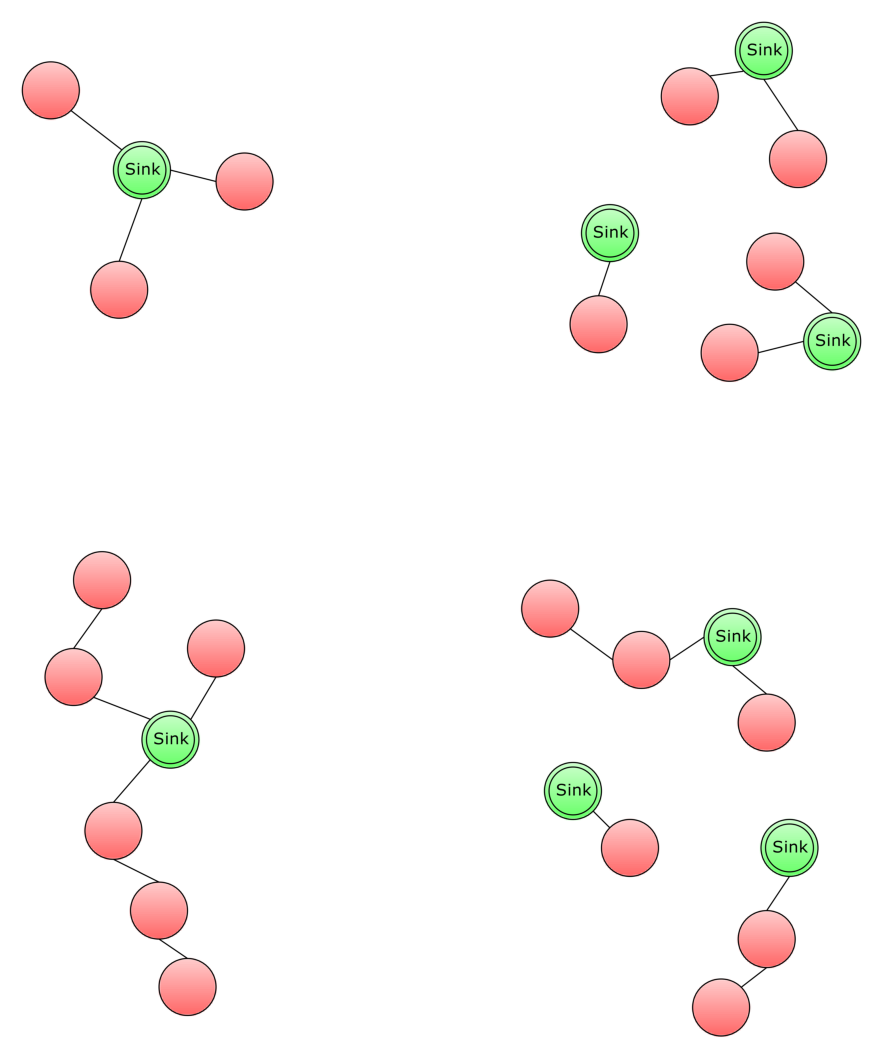
\includegraphics[scale=0.8]{img/types_of_wsn.pdf}
	\end{center}
	\caption{\small \itshape{Types of WSNs: single-hop/single-sink
	(top left), single-hop/multi-sink (top right), multi-hop/single-sink
	(bottom left) and multi-hop/multi-sink (bottom right)}}
\end{figure}

Wireless Sensor Networks can have several features:
\begin{itemize}
	\item \emph{Self-configuration}: the nodes' ability to form a network
		using pre-established high-level rules but no user interaction
		or configuration\cite{prehofer2005self}.
	\item \emph{Fault tolerance}: the network's ability to recover after
		the failure of one or more nodes and maintain network
		integrity\cite{koushanfar2002fault}.
	\item \emph{Energy efficiency}: power consumption must be as low as
		possible in order to increase network lifetime.
	\item \emph{Low cost}: nodes must have a low acquisition and
		maintenance cost in order to become a viable alternative to
		traditional wired sensor networks.
\end{itemize}

% ********** End of Introduction **********
